\documentclass{techbrief}

\title{Tech Brief}
\title{Activities}
\date{August 31}
\event{Special Report}

\usepackage{lipsum}

\begin{document}
\newgeometry{margin=1cm,headheight=3cm,includehead,includefoot}
\pagestyle{main}
\thispagestyle{title}
\pagenumbering{gobble}
\noindent

\lettrine[lines=2]{X}{imera} made a significant impact at \textit{MathFest
    2024},
capturing the attention of many attendees. Our booth, with a strategic location
in
the exhibit hall, was a focal point of the event. Throughout the conference, we
showcased Ximera's capabilities and discussed our future plans.
Eight dedicated members of the Ximera team were on-site, including Anna Davis,
Alex Dempsey, Jim Fowler, Austin Jacobs, Nick Kronic, Jason Nowell, Jenny
Sheldon, and Bart Snapp.

\begin{xframe}
    \textbf{The Ximera booth} was open Wednesday 6:30pm--8:30pm, Thursday
    9am--6pm, and Friday 9am--5pm. Our corner booth, easily visible from the
    entrance, attracted participants with a vibrant slide show on a 100-inch
    screen.
    \begin{center}
        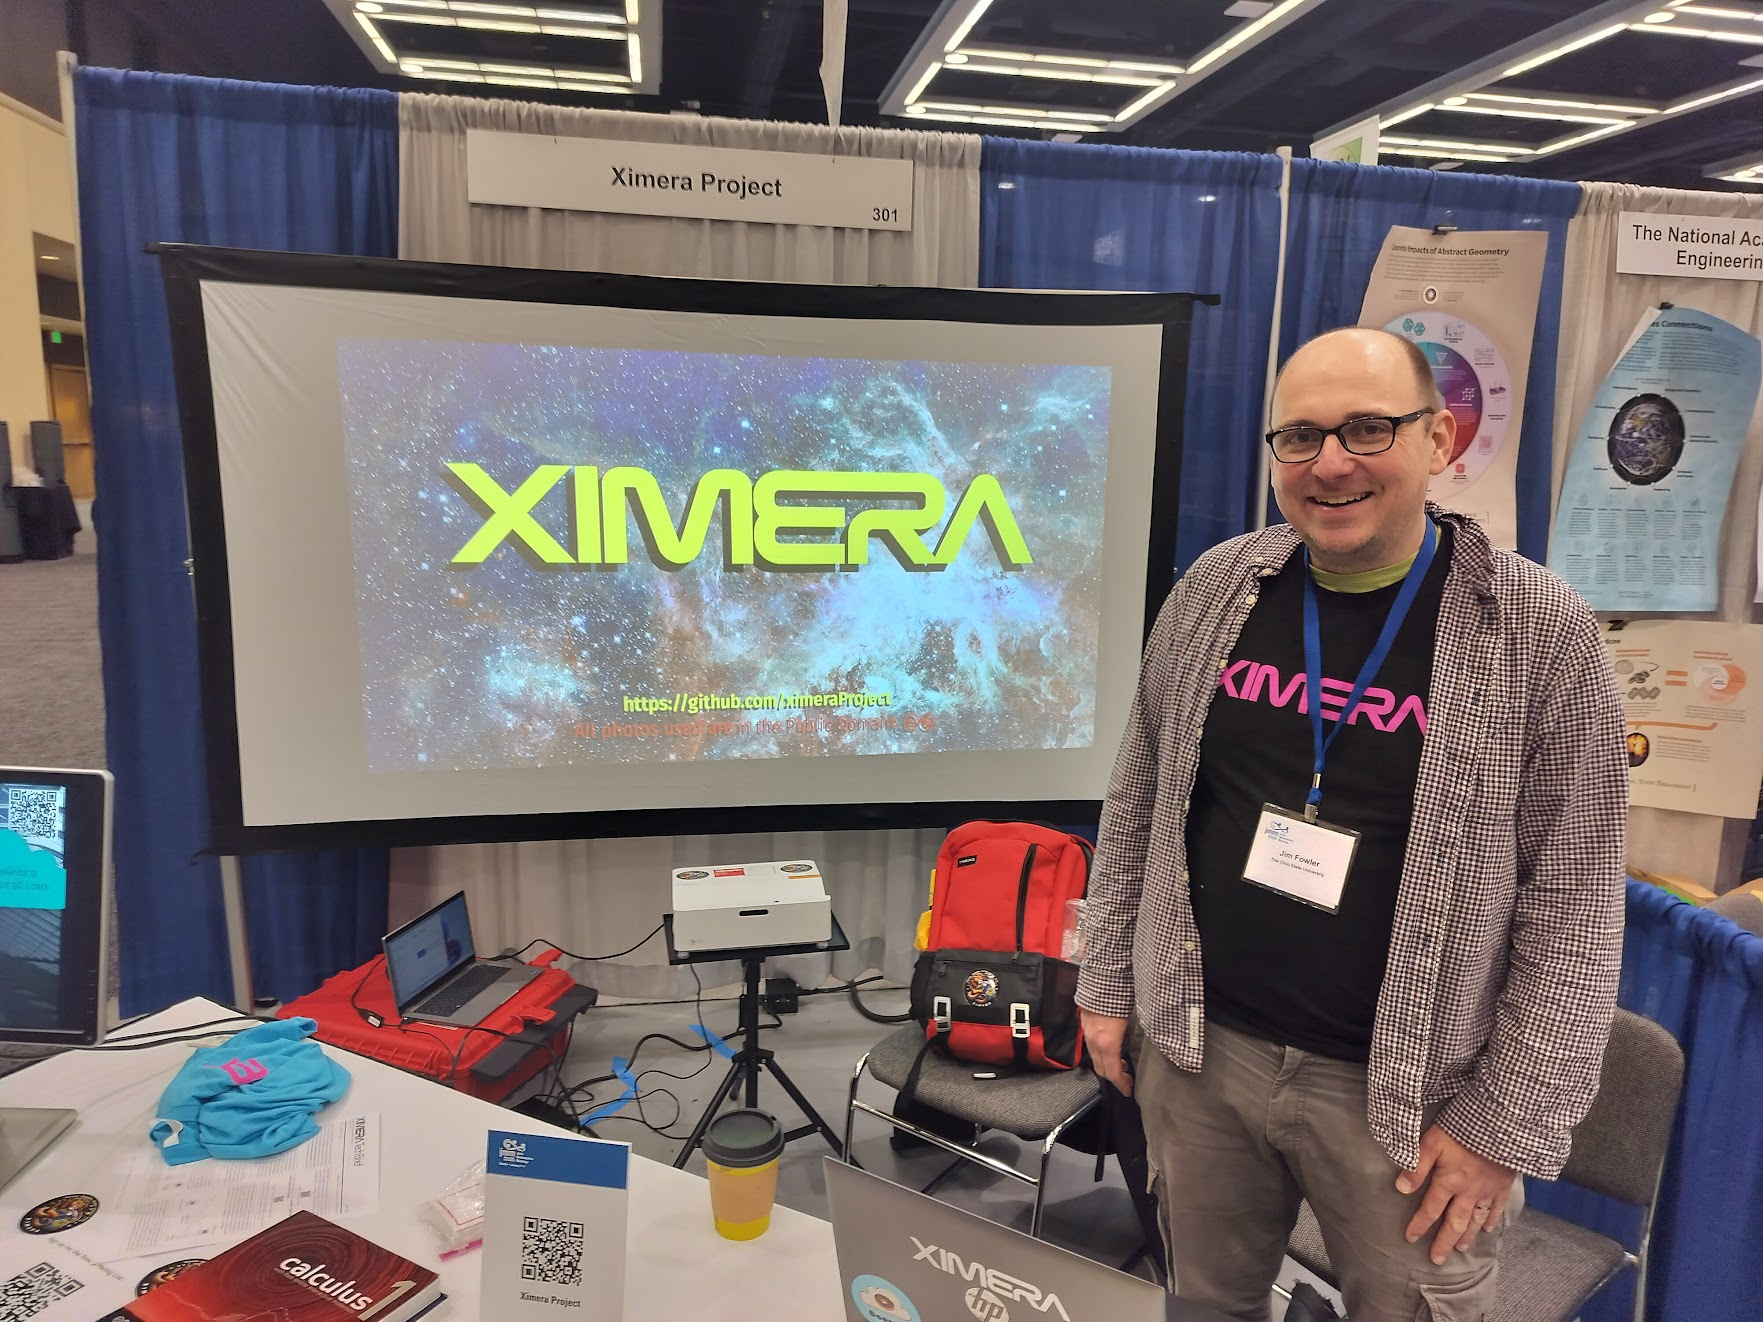
\includegraphics[width=.9\textwidth]{booth.jpg}
    \end{center}
    On our table, a computer monitor was used to display a video showing Ximera
    in action.
    We also had bound demonstration copies of our calculus texts and
    \textit{Linear Algebra: An Interactive Approach} by Anna Davis and Paul
    Zachlin.
    We gave away Ximera stickers and buttons. The stickers were a hit.

    We currently have:
    \begin{center}

        
\includegraphics[width=.2\textwidth]{../../missionPatch/missionPatch.png}
        \qquad

        \includegraphics[width=.4\textwidth]{../../criticalMathItem/criticalItem.pdf}
    \end{center}
    Please contact us if you would like Ximera stickers and I will fill your
    order with some degree of accuracy.
\end{xframe}

\begin{xframe}
    \textbf{Presentations featuring Ximera} were popular talks and were left
    with `standing-room only.'

    On Tuesday, A.\ Davis presented a wonderful Math Circle activity
    \textit{Lines of Sight} authored in Ximera.
    In this activity young mathematicians are shown pictures of railroad tracks
    and then asked a number of questions ranging from the simple to the
    seemingly
    impossible. We won't spoil it, but at the end, there's definitely an
    \textit{Ah-ha! Math Moment}.

    On Friday, J.\ Fowler and B.\ Snapp gave a lively presentation to
    participants interested in open-source resources for the classroom. The
    talk
    was
    a HIT! Participants  definitely found a new interest in Ximera.

    Combined, the presentations had an audience of around 100 participants.
\end{xframe}
%% WIM and graphics /preamble

\begin{xframe}
    \textbf{Ximera deployment} was improved along with its documentation. The
    Ximera team worked tirelessly to enhance our deployment process and its
    documentation. Team members, including J.\ Nowell, A.\ Jacobs, A.\ Davis,
    A.\ Dempsey, and B.\ Snapp, were often seen fine-tuning the deployment,
    addressing minor bugs, and significantly improving the documentation.
\end{xframe}

\begin{xframe}
    \textbf{New friends} were made! In all we gave out around 200 Ximera
    TechBriefs and added nearly 20 emails to our mailing list.	Several
    participants expressed interest in converting their current \LaTeX\ content
    into Ximera, opening doors for future collaborations.
\end{xframe}

\begin{xframe}
    {\sffamily\bfseries The Joint Mathematics Meetings} are from January 8--11
    in Seattle, Washington. We will be running a Ximera booth in the exhibit
    halls,and applying to give talks in the sessions. The deadlines for
    presentations is September 10, 2024. If you are interested in representing Ximera at the
    Joint Meetings, consider applying for a Ximera Flash-Grant to support your
    travel.
\end{xframe}

\begin{xframe}
    \textbf{Funding for the Ximera Project} is provided by
    a U.S.\ Department of Education Open Textbooks Pilot Program grant in the
    amount of \$2,125,000, from 2024--2026, with no external funding. In the
    past, the Ximera Project has
    also received support from NSF Grant DUE-1245433, the Shuttleworth
    Foundation, the Ohio State University
    Department of Mathematics, and the Affordable Learning Exchange at OSU.
\end{xframe}

\end{document}